\chapter{基于移动运营商数据的用户上网行为分析}
\label{cha:interest}

%%%\newdef{definition}{Definition}



\section{相关工作}
\label{interest:sec:relatedwork}

基于互联网使用记录的用户兴趣和行为挖掘长久以来便是一个热门的课题\cite{kdd00kosala}\cite{kdd00srivastava}\cite{widm01Mobasher}。 White等\cite{sigir09white}使用5种不同的上下文信息来建模用户兴趣,并依据用户兴趣进行推荐服务。Nasraoui等\cite{tkde08nasraoui} 通过追踪用户在某一特定网站的档案和行为,针对这一网站研究了用户的行为模式。也有些研究人员使用聚类方法来发现用户的类型\cite{icina10xu}\cite{kdex99mobasher}。然而,这些方法或者从用户的角度出发,将用户聚成不同的类型;或者从网站的角度出发,将网站URL聚合成不同的类型,而不是使用层次化多为聚类方法,在统一的模型中同时发现用户类型和网站类型。 

随着移动互联网在人们对互联网的总使用量中所占比重的不断增大,移动互联网中的用户行为也获得了研究者的关注\cite{pm2hw2n12almutairi}。Cui等\cite{www08cui}通过上下文获取方法,描述了人们在移动设备上使用互联网的方式,并分析了其中的上下文因素和用户行为模式。Tseng等\cite{ist06tseng}基于地理位置轨迹挖掘用户在移动互联网系统中的行为模式,并通过模拟实验进行了验证和分析。Phatak等\cite{fuzzy02phatak} 提出了基于距离矩阵的针对网站URL和用户的模糊聚类方法,并据此进行用户的建模和推荐服务。Do等\cite{mum10do}使用手机应用使用情况进行用户模式挖掘,其中包含了移动互联网使用记录。Verkasalo\cite{puc09verkasalo}手机了手持设备数据(包含移动互联网使用记录),从统计学角度分析了移动服务使用情况中的上下文模式。这些研究大多使用手机手机的数据,这些数据对于面向用户个体的行为分析可以胜任,但由于其难以规模化,限制了方法应用的规模和分析结果。本文提出的方法从移动运营商的角度,使用移动运营商的用户网络使用记录进行用户行为的分析与挖掘,保证了规模性型和全面性。

\section{数据描述}
\label{interest:sec:data}

本文使用的数据为某一移动运营商蜂窝网络(包括2G与3G)中的移动互联网使用记录(HTTP请求记录)。数据集覆盖的地理区域为北京市城区的一部分,集中在东城区和朝阳区的一部分,覆盖的区域面积约为40平方公里。区域内包含了故宫、天安门等热门景点,以及国贸、三里屯等重点商圈。区域内的常住居民约为90万。本数据集的时间跨度为2012年10月24日到2012年11月14日。

数据集中的每一条记录对应于一个发生在运营商蜂窝网络中的HTTP请求/响应对,数据的主要结构见表\ref{interest:tab:fields}。

\begin{table}
\centering
\caption{运营商数据集列结构}
\label{interest:tab:fields}
\begin{tabular}{|c|c|l|} \hline
名称 & 数据类型 & 描述\\ \hline
用户ID & 字符串 & 用户的唯一标识符\\ \hline
纬度 & 浮点数 & 移动基站的纬度\\ \hline
经度 & 浮点数 & 移动基站的经度\\ \hline
请求时间 & 时间 & 请求发生的时间\\ \hline
主机地址 & 字符串 & 被请求的主机的地址\\ \hline
内容类型 & 字符串 & HTTP协议中的ContentType域 \\
\hline\end{tabular}
\end{table}

\textbf{数据概览.} 数据集中包含的完整记录共有 \textbf{578,134,225} 条。对于数据的清理,采用了如下方法:
\begin{inparaenum}[\itshape 1\upshape)]
\item 数据分析关注于用户行为, 故使用\textit{内容类型}域将所有附加资源请求过滤掉(包括CSS,JavaScript以及附加图片等)。
\item 根据\textit{主机地址}域,将无意义的请求(如地址全是问号)过滤掉。
\end{inparaenum}
经过数据清洗之后,共有\textbf{66.823\% (386,332,325条)}的记录被保留下来。

\textbf{用户.} 数据集中出现过的独立用户数为\textbf{3,524,929}。图\ref{interest:fig:usertotalcountdist}中展示了用户的总请求数的分布情况。从图中可以看出,\textbf{40\%}的用户一周内发出的请求书少于10个;超过\textbf{95\%}的用户每周的请求书少于1,000个。每用户每周的平均请求数位\textbf{137.27}。

\begin{figure}
\centering
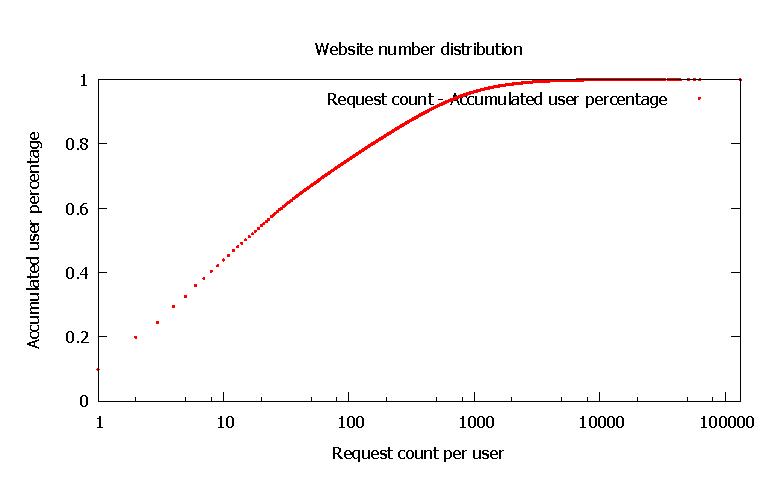
\includegraphics{user_conncount}
\caption{每用户请求数对应的用户数}
\label{interest:fig:usertotalcountdist}
\end{figure}

\textbf{主机地址.} 数据集中共出现了\textbf{363,841}个不同的主机地址。然而,只有\textbf{40.12\%}的主机地址被多于1个用户访问过。 按访问数降序排列,排名前990的主机地址占据了总记录数的97.877\%,而排名前10的主机地址占据了总记录数的58.1\%。可以看出,与传统桌面互联网相比,移动互联网中的网站/服务使用情况要集中得多。

\textbf{地理位置.} 数据集共涵盖了856个独立的蜂窝基站,每个基站由其经纬度唯一确定其位置。原始的基站数据对于用户行为建模来说意义不大,本文将基站聚类为地理区域后加入用户行为模型中。(详见第\ref{interest:sec:region}章)


\section{地理区域发现}
\label{interest:sec:region}
地理位置在移动互联网使用的上下文中占有重要的地位。用户所访问的网站与该访问行为发生的地点有着自然的联系,比如,相较于在住宅区的用户(通常在家里),CDB区域的用户更有可能通过手机使用本地搜索来查询附件的餐馆信息;与工作地点相比,人们更可能在家里使用手机阅读等等。
数据集中原始的地理位置信息(基站)力度太细,蕴含的语义信息太少。因此,在地理位置相关的挖掘中,通常把地点看成更大的地理实体的一部分,如地理区域\cite{env07park},或者轨迹\cite{www10zheng}\cite{debu10zheng}。在移动互联网使用的情境中,上网行为发生的所在地点的地理区域功能更为重要,本研究中,将位置点聚合成地理区域,后者作为用户行为模型中的因素考虑。
数据集中提供原始位置点(经纬度)为蜂窝基站的位置,基站覆盖范围(即位置精度)为50-150米。
\begin{definition}
\textbf{功能区域}. 城市的一个地理功能区域(以下简称为区域),定义为提供一个特定集合的城市功能的最小地理范围。某一区域所提供的功能集合对于绝大多数居民来说是一样的。
\end{definition}
如上定义的功能区域通常会包含数目不定的若干个基站,需要将基站聚类成区域,并且找出每个区域的功能特征。
\subsection{聚类算法}
本研究使用一个改进的DBSCAN算法来进行地理位置的聚类。

DBSCAN算法中的类簇定义基于密度可达性。算法中有两个参数:$\epsilon$和$MinPts$,通过这两个参数定义点的邻域($\epsilon-neighborhood$),从而判断密度可达性。下面介绍DBSCAN算法中的基本概念:

点$p$的$\epsilon-neighborhood$用$N_\epsilon(p)$来表示,定义为:$N_\epsilon (p)=\{q \in D|dist(p,q) \leq \epsilon \}$。对于聚类,直观的做法是,对于类簇中的所有点,该点的$\epsilon-neighborhood$中至少包含$MinPts$个点。
一个类簇是数据库中所有点集合的一个子集,其中包含的点满足两个属性:其中所有的点之家俩俩之间密度相连;如果某个点与类簇中的任意一个店密度相连,则其也属于这个类簇。\cite{ester1996density}

本文改变了$\epsilon-neighborhood$的计算方法。本研究中,$\epsilon-neighborhood$的定义中包含基于三种相似度/距离的限制规则:(A和B是两个基站)
\begin{itemize}
	\item 记录相似度$sim\_r$。$sim\_r$表示A和B在记录数量上的相似程度。处于同一区域内的基站,由于其功能的相似性,一天内不同时间段间记录数的分布情况也应具有较高的相似性。
	\item 迁移记录相似度$sim\_m$。如果用户$u$在A范围内有一条访问记录,短时间内在B范内又有一条访问记录,则称此为一次\textit{迁移记录}。迁移记录的多少体现了两个基站之间人员的流动成都,也体现了二者联系的紧密性。
	\item 地理距离$dg$。$dg_{(A,B)}$表示A与B之间的地理距离(单位为\textit{米})。
\end{itemize}
$sim\_r$的计算方法如下。考虑到用户访问行为在工作日和周末之间存在差别,因此对二者分别对待。以\textit{1小时}作为时间槽,共能得到48个关于一个基站的统计数据:工作日数据$vd_(A,i)$以及周末数据$ve_(A,i)$(i的取值范围是 0 到 23,代表24个小时)。$sim\_r_{(A,B)}$的计算见式\ref{interest:equ:simr}。
\begin{equation}
\label{interest:equ:simr}
	sim\_r_{(A,B)} = \frac{\sum_{i=0}^{23}{\left(\frac{vd_{(A,i)}}{vd_{(B,i)}} + \frac{ve_{(A,i)}}{ve_{(B,i)}}\right)}}{48}
\end{equation}

对于迁移记录相似度,A与B之间的总迁移记录数便能够反映二者之间联系的紧密性,不需要更细致的数据。用$m_{(A,B)}$来表示A与B之间的迁移记录总数,则$sim\_m$可按如下方法计算:

\begin{equation}
	sim\_m_{(A,B)} = \frac{m_{(A,B)}}{v_A}
\end{equation}
其中$v_A$为A基站内的所有记录总数。

值得注意的是,如此定义的相似度并不是对称的,也即$sim\_m_{(A,B)} \neq sim\_m_{(B,A)} $。在计算$\epsilon-neighborhood$的时候,双向的迁移记录相似度均被作为条件考虑。 

地理距离上的限制条件$dg$是可调整的。由于基站的密度在不同区域间存在很大差别,为此定义了两个级别的阈值$DG_s$与$DG_l$($DG_s < DG_l$),并且根据基站临近的其他基站数目来动态调整应用于$dg$的阈值。 

最终,综合三种距离/相似度上的限制来确定某一基站的$\epsilon-neighborhood$,详见算法\ref{interest:alg:neighber}。
如果计算得到的A基站的$\epsilon-neighborhood$不为空,则将A视为DBSCAN中的核心点
\begin{algorithm}
%\SetAlgoLined
% \KwIn{基站A;\\ 
% 所有基站的集合$\mathbf{C}$;\\
% 阈值的默认取值$SIM\_R_0$,$SIM\_M_0$,$DG_s$以及$DG_l$;
% 参数$MinPts$}
% \KwOut{${\epsilon-n}_A$,即基站A的$\epsilon-neighborhood$内的所有基站}

% 初始化 ${\epsilon-n}_A$ 为空集;
\KwIn{Cellular tower A;\\ 
Set of cellular towers $\mathbf{C}$;\\
Default values of thresholds $SIM\_R_0$, $SIM\_M_0$, $DG_s$ and $DG_l$;
Value of parameter $MinPts$}
\KwOut{${\epsilon-n}_A$, containing all other cellulars in the $\epsilon-neighborhood$ of A}

Initialize ${\epsilon-n}_A$ as empty set;

Initialize thresholds $SIM\_R \leftarrow SIM\_R_0$, $SIM_M \leftarrow SIM\_M_0$, $DG \leftarrow DG_s$

\For{Each other cellular $B \in \mathbf{C}$}{
		\If{A and B are neighbors under current threshold configuration}{
			Add B to ${\epsilon-n}_A$;
		} 
}
\If{${\epsilon-n}_A$ is empty \textbf{and} $DG = DG_s$}{
		$DG \leftarrow DG_l$;
		
		Restart the For loop
}
\If{Size of ${\epsilon-n}_A \geq MinPts$}{
	Add A to ${\epsilon-n}_A$;
} \Else {
	Reset ${\epsilon-n}_A$ to empty;
}
Return ${\epsilon-n}_A$;
\caption{计算某一基站的$\epsilon-neighborhood$}
\label{interest:alg:neighber}
\end{algorithm}

\begin{algorithm}
%\SetAlgoLined
\KwIn{Cellular tower A and B (A $\neq$ B); 

Values of thresholds $SIM\_R$, $SIM\_M$, and $DG$}
\KwOut{Whether B is in the $\epsilon-neighborhood$ of A}
	\If{$dg_{(A,B)} > DG $}{
		Return FALSE;
	}\Else{
		Compute $sim\_r_{(A,B)}$ and $sim\_m_{(A,B)}$;
		
		\If{$1 < sim\_r_{(A,B)} \leq SIM\_R$ \textbf{or} $1 < sim\_r_{(B,A)} \leq SIM\_R$}{
			Return TRUE;
		}\ElseIf{$1 < sim\_m_{(A,B)} \leq SIM\_M$ \textbf{or} $1 < sim\_m_{(B,A)} \leq SIM\_M$}{
			Return TRUE;
		}
	}

\caption{判断两个基站是否临近(密度可达)的算法}
\label{interest:alg:pair}
\end{algorithm}

\subsection{聚类结果}
使用上述算法和参数配置,717个基站被聚类成126个区域,剩余的139个基站为单基站区域,总计得到265个区域。所得区域在地图上的分布见图\ref{interest:fig:regions}。

\begin{figure}
\centering
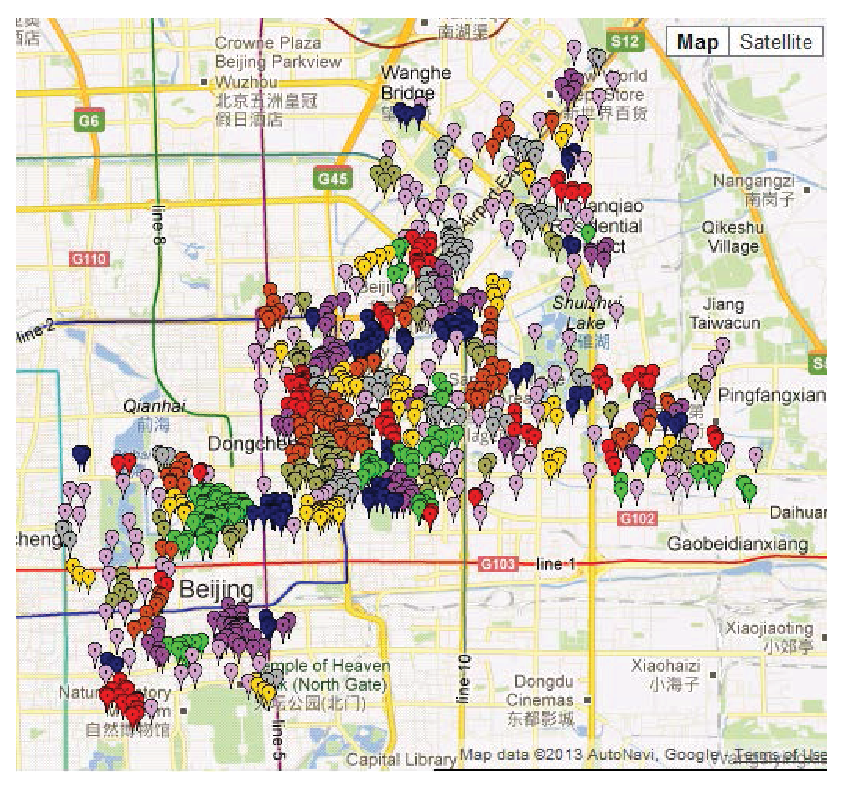
\includegraphics{regions}
\caption{以区域内基站标识的区域分布图}
\label{interest:fig:regions}
\end{figure}

为评估算法的分类结果,实验中试用了手工标注的每个基站所属的区域功能类型(数据来源于移动运营商)。
区域类型被进一步分成5个类别:\textit{居住区,工作区,活动区,学校}以及\textit{其他}。使用这些数据来分析126个聚类所得区域的准确性。

每个聚类所得区域被赋予一个分数。首先,将本区域内出现频率最高的类型作为本区域的功能类型。而后计算本区域内属于此类型的基站所占的比例$p$。
如果$p \geq 0.5$,表示此区域半数以上的基站具有同样的功能类型,那么这个区域的分数则为$p$。反之,如果$p < 0.5$,则认为这个区域的聚类不合理,其分数为0。

最终,126个区域中有99个区域的分数大于0.5,所有区域的平均得分为0.66。

以故宫周围区域为例进行说明(见图\ref{interest:fig:fob}):可以看到,故宫内的基站和王府井地区的基站被成功的分到了不同的区域内。然而,故宫内的基站也被分成了两个区域:北侧和南侧。这是因为故宫中央的基站过于稀疏,无法将南北两个区域连接起来。

\begin{figure}
\centering
\scalebox{0.75}{
	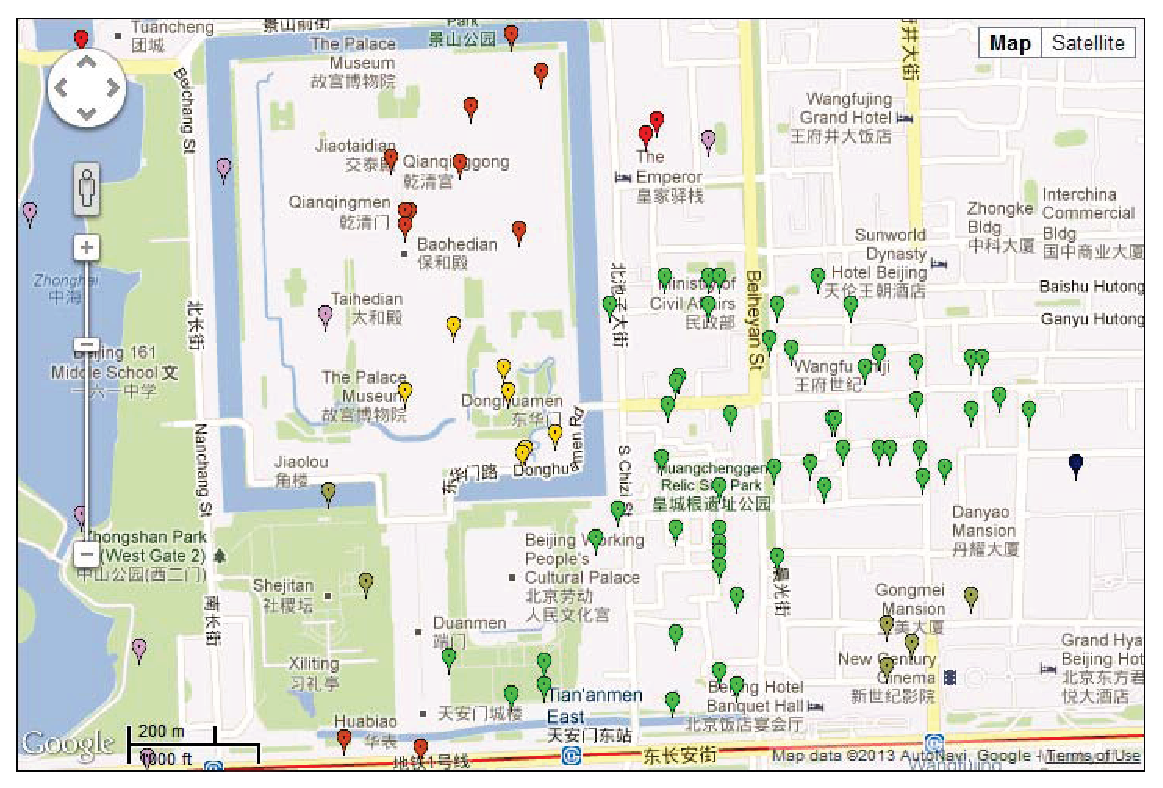
\includegraphics{forbidden}
}
\caption{故宫附近的区域分布情况}
\label{interest:fig:fob}
\end{figure}

针对27个``不合理''区域进行分析,人工检查其中的基站发现,其中的绝大部分基站的类别标识为``高密度居民区''以及``企业办公区'',可以推断这些地区包含综合功能大厦,低层用于商业活动,高层作为居住区。按照前文对于区域的定义,这些区域也是符合要求的混合功能区域,在模型中可以作为一个整体对待。故总的来说,聚类结果对于建模需求来说是可靠的。


\section{用户兴趣发现模型}
\label{interest:sec:uri}
首先给出``用户兴趣''的定义。

\begin{definition}
\label{interest:def:ui}
\textbf{用户兴趣}. 某个户的兴趣表示该用户感兴趣、喜欢浏览或使用的某一特定类型的网站或服务。一个用户可能有多种不同的兴趣,每个兴趣有一个权值,代表该用户对这个兴趣的喜爱程度。另一方面,用户兴趣也可能表示网站或服务的风格而不是类型,一个网站也可能属于多种不同的用户兴趣类型。
\end{definition}

为了从移动互联网使用记录中抽取隐含的用户兴趣,,本文提出了一个基于LDA(Latent Dirichlet Allocation)的概率话题模型方法。在这个模型中,抽取出来的隐含层即表示定义\ref{interest:def:ui}中的\textit{用户兴趣}。

话题模型是目前在文本挖掘中常用的建模方法,用以发现一个文档集中隐含的``话题''层。LDA(Latent Dirichlet Allocation)\cite{jmlr03blei}是一个目前最常用的话题模型,而且被扩展应用于除了词之外的其他文档属性(作者,会议,等等)\cite{kdd04steyvers}\cite{kdd08tang}\cite{kdd12tang}。也有研究者将LDA及其扩展模型应用于用户行为模式的发现\cite{tist11farrahi}。LDA是一个非监督的生成模型,将一篇文档的生成过程(每个词的撰写过程)分成两个阶段:第一阶段为根据文档上的话题分布选择一个话题;第二阶段为根据话题上的次分布选择一个词。

使用访问的网站集合来表示用户,类似LDA中的文档,而后对其进行话题模型建模。

\subsection{网站发现}
\label{interest:sec:website}
本章将介绍从原始的移动互联网HTTP访问记录抽取网站的方法。

首先,给出一些模型中常用概念的定义。

\begin{definition}
\textbf{用户}:用户在数据集中由\textit{用户ID}唯一标识,并唯一对应于一个使用移动互联网的自然人(一个手机号码),无论其使用的是否为同一个联网设备。
\end{definition}

\begin{definition}
\label{interest:def:host}
\textbf{主机}:主机即HTTP请求中的被请求主机,由主机地址(URL)唯一确定。此地址可能是,也可能不是用户/应用直接访问的地址。
\end{definition}

根据常识以及对数据的观察,第三级及以上的域名(如果此主机地址的顶级域名为国家/地区域名,二级域名为通用域名,如\textit{.com.cn},则是第四级及以上的域名)在标识不同的网站/服务上并不起作用。\footnote{如QQ,Baidu等超大型移动互联网服务公司的域名除外,它们下属的子域名可能会提供完全不同的服务。这种情况下多加一级的域名会被保留下来。}基于上述观察,原始数据经过一次预处理,将URL中不起作用的部分移除,保留下来的部分作为主机地址唯一标识主机。实验表明,没有这一步预处理的情况下,来自同一根域名的不同地址会在话题模型中形成干扰。

网站与被地址唯一标识的主机并不完全等同(参见定义\ref{interest:def:host})。当用户访问某一网站时,可能会对不同的主机地址发出多个请求。因此,需要首先将主机聚类,每个类代表一个网站。

\begin{definition}
\textbf{网站}. 一个网站代表一个给用户提供内容或服务的独立主体,可能使用多个不同的主机地址。 
\end{definition}

网站和主机并没有很强的关联关系。例如,网站\textit{qq.com}是一个腾讯旗下的知名门户网站,而其子域名\textit{t.qq.com}则是腾讯旗下的微博网站,二者并不属于同一网站;另一方面,\textit{t.sina.com.cn}和\textit{weibo.com}主机地址完全不同,但都是新浪微博的地址,所以按照上述定义,他们应属于同一网站。

将主机聚类成网站的算法描述如下。首先,将每个主机看成一个向量$H_i: <C_{h_i, u_1}, C_{h_i, u_2},...,C_{h_i, u_n}>$,其中$C_{h_i, u_j}$是用户$j$向主机$i$发出的请求数。而后,使用这一向量表示计算主机俩俩之间的余弦相似度。之后设定一个阈值$\alpha$,将所有相似度高于$\alpha$的主机对儿看成同一网站内的主机。

实验中,使用了从0.1到0.9范围内的不同$\alpha$值,不同阈值与所得的网站数量的对应关系见图\ref{interest:fig:websitecount}。由于在用户行为模型中,网站被视为一种最小单元,故在网站发现的过程中,应更关心聚类的准确度,所以倾向于选择更大的$\alpha$值。 基于图中曲线的形状,以及对聚类结果的观察,最终选定的$\alpha$值为\textbf{0.5}。在此阈值下,生成的网站示例如:``Website No.580: wikipedia.org, wikimedia.org'',``Website No.357: adsmogo.mobi, adsmogo.org, adsmogo.com''。

使用\textbf{0.5}作为阈值共得到924个网站。其中大部分的网站仍然只包含一个主机,最大的一个聚类包含5个主机。

\begin{figure}
\centering
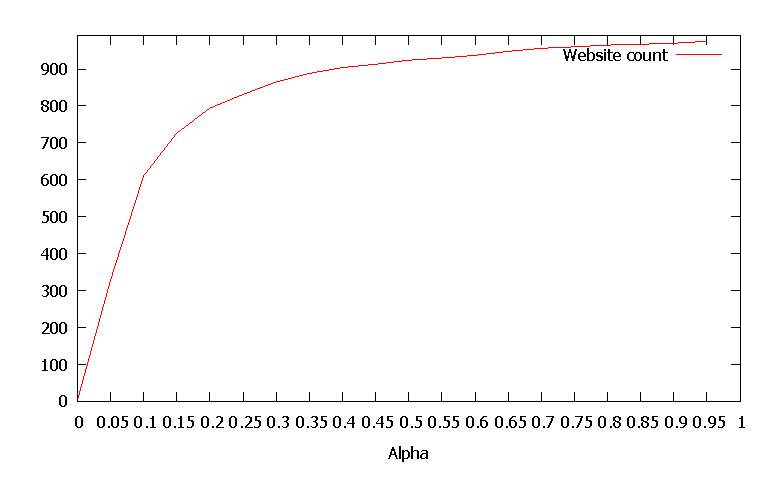
\includegraphics{alpha_websitecount}
\caption{网站数量与聚类阈值的关系图}
\label{interest:fig:websitecount}
\end{figure}

\subsection{用户的网站向量表示} 

模型中将用户视为文档,将网站视为词。网站在用户表示中的每一次出现(即该用户访问了该网站)都被关联以一个区域,对应与该次访问行为所发生的区域。

由于原始的HTTP记录并不能忠实地反映用户的行为,在生成表征用户的向量时,对原始记录进行了转换处理。处理过程如下:
首先,将一天分成48个半小时跨度的时间槽,并将每个时间槽作为表示用户行为的稳定时间段(即半小时内用户的网站访问行为基本稳定)\cite{tist11farrahi}。而后,对于每个用户$u$以及每个时间槽$t$,排名前三的访问量最大的网站被视为在这个时间槽内被该用户``访问''。对于每个被访问的网站$w$,用户$u$在时间槽$t$内访问$w$的所有记录中出现次数最多的区域被视为关联到这次$w$的访问的区域。于是,一个用户可以被如下表示:$U = \{{<w_{ui}, r_{ui}, c_{u,w_{ui},r_{ui}}>}\}$,其中$c_{u,w_{ui},r_{ui}}$是用户$u$访问$<w_{ui}, r_{ui}>$的次数。

\subsection{用户-区域-兴趣(URI,User-Region-Interest)模型}
本文将用户,网站,地理区域,以及用户兴趣综合考虑,用同一的生成模型进行建模。按对``用户兴趣''这一隐含层的实际解释不同,以及在生成过程中考虑\textit{区域}的策略的不同,提出了两种不同的生成过程,以及对应的两种不同的URI模型。

\textbf{URI1模型} 在第一个模型(URI1)中,隐含的``用户兴趣''层被视为用户频繁的网络使用模式,与用户一方的联系更为紧密。每个用户有一个``用户兴趣''的分布,这一份不与地理位置无关;同时,每个``用户兴趣''中,针对每个区域有一个不同的网站分布。这一模型下的生成过程如下(见图\ref{interest:fig:uri}):
\begin{enumerate}
	\item 对于每个用户$u$,根据狄利克雷先验$\alpha$生成$\theta_u$;
	\item 对于每个用户兴趣$z$, 根据狄利克雷先验$\beta_z$,对每个区域$r \in R$生成$\phi_{(z,r)}$;
	\item 对于用户$u$内的每此网站访问$w_{ui}$:
	\begin{itemize}
		\item 根据多项分布$theta_u$生成$z_{ui}$;
		\item 根据多项分布$\phi_(z_{ui},r_{ui})$生成网站$w_{ui}$。
	\end{itemize}
\end{enumerate}

模型的参数估计部分使用吉布斯抽样(Gibbs sampling)方法\cite{nas04griffiths}。简单化考虑,对超参数取值$\alpha$和$\beta$采取了固定取值(如,$\alpha = 50 / T$, $\beta = 0.01$)。使用吉布斯抽样方法来估计$w$,$z$以及$r$的后验概率分布,而后用结果来估计$\mathbf{\theta}$以及$\mathbf{\phi}$。
后验概率的计算方法是:
	\begin{equation}
	P(z_{ui}|\mathbf{z_{-ui}},\mathbf{w}, \mathbf{r}, \alpha, \beta) \propto
	  \frac{m^{-ui}_{u,z_{ui}} + \alpha_{z_{ui}}}{\sum_{z}{(m^{-ui}_{u,z} + \alpha_z)}}
		\frac{n^{-ui}_{z_{ui},r_{ui},w_{ui}} + \beta_{w_{ui}}}{\sum_{w}{(n^{-ui}_{z_{ui},r_{ui},w} + \beta_w)}}
\end{equation}
其中$m_{u,z}$表示在吉布斯抽样中,兴趣$z$被分配给用户$u$的次数,$n_{z,r,w}$表示兴趣$z$在区域$r$内被分配给用户$w$的次数。上标$-ui$表示此技术并不包含当前的实例。

抽样过程收敛后,多项分布参数$\theta$和$\phi$使用如下方法计算:

\begin{equation}
	\theta_{u,z} = \frac{m_{u,z} + \alpha_z}{\sum_{z'}{(m_{u,z'} + \alpha_{z'})}}
\end{equation}
\begin{equation}
\label{interest:equ:phi}
	\phi_{z,r,w} = \frac{n_{z,r,w} + \beta_w}{\sum_{w'}{(n_{z,r,w'} + \beta_{w'})}}
\end{equation}

\begin{figure}
\centering
\includegraphics{uri}
\caption{User-Region-Interest (URI) 模型1 的盒图表示}
\label{interest:fig:uri}
\end{figure}

\textbf{URI2模型} 在第二个模型(URI2)中,隐含的``用户兴趣''层被看成是常见的经常同现的网站集合,与网站的联系更为紧密。每个``用户兴趣''上有一个所有网站的分布,这一分布与地理位置无关;而每个用户上的``兴趣''分布则与地理位置有关。URI2的生成过程如下(见图\ref{interest:fig:uri2}):
\begin{enumerate}
	\item 对于每个用户$u$, 根据狄利克雷先验$\alpha_u$,对每个区域$r \in R$生成$\theta_{(u,r)}$;
	\item 对于每个用户兴趣$z$, 根据狄利克雷先验$\beta$生成$\phi_z$;
	\item 对于用户$u$内的每此网站访问$w_{ui}$:
	\begin{itemize}
		\item 根据多项分布$theta_{(u,r_{ui})}$生成$z_{ui}$;
		\item 根据多项分布 $\phi_{z_{ui}}$生成网站$w_{ui}$。
	\end{itemize}
\end{enumerate}

与URI1模型类似,使用吉布斯抽样方法来估计模型参数。超参数同样被设定为固定值(如$\alpha = 50 / T$,$\beta = 0.01$),后验概率的计算方法为:
	\begin{equation}
	P(z_{ui}|\mathbf{z_{-ui}},\mathbf{w}, \mathbf{r}, \mathbf{\alpha}, \mathbf{\beta}) \propto
	  \frac{m^{-ui}_{u,r_{ui},z_{ui}} + \alpha_{z_{ui}}}{\sum_{z}{(m^{-ui}_{u,r_{ui},z} + \alpha_z)}}
		\frac{n^{-ui}_{z_{ui},w_{ui}} + \beta_{w_{ui}}}{\sum_{w}{(n^{-ui}_{z_{ui},w} + \beta_w)}}
\end{equation}

$\theta$和$\phi$的估计方法为:

\begin{equation}
\label{interest:equ:theta2}
	\theta_{u,r,z} = \frac{m_{u,r,z} + \alpha_z}{\sum_{z'}{(m_{u,r,z'} + \alpha_{z'})}}
\end{equation}
\begin{equation}
	\phi_{z,w} = \frac{n_{z,w} + \beta_w}{\sum_{w'}{(n_{z,w'} + \beta_{w'})}}
\end{equation}

\begin{figure}
\centering
\includegraphics{uri2}
\caption{User-Region-Interest (URI) 模型2 和盒图表示}
\label{interest:fig:uri2}
\end{figure}


\section{实验}
\label{interest:sec:exp}

本章将展示在数据集上应用模型的结果,并给予实验结果进行分析讨论。
\subsection{实验数据}
\label{interest:sec:expdata}
实验使用的数据描述见第\ref{interest:sec:data}章。首先,实验选取了访问量前990的网站,它们只占网站总数的0.27\%,却占据的总访问量的97.877\%。此后,对于数据集中出现的所有用户,按照前文描述生成器网站向量表示。对于生成的用户集合,将其中包含5个以上不同的网站-区域对的用户是为活跃用户。将不活跃用户过滤掉以后,保留的活跃用户数为\textit{469,297},占原用户总数(\textit{3,524,929})的13.31\%。在所有的\textit{386,332,325}记录中,经过两步过滤,\textit{263392870 (68.18\%)}条记录保留了下来。

每个时间槽内的活跃用户数见图\ref{interest:fig:usercount}。从图中可以看出,在经过表示形式转换之后,曲线能够很好的和现实生活中的生活模式相匹配。

\begin{figure}
\centering
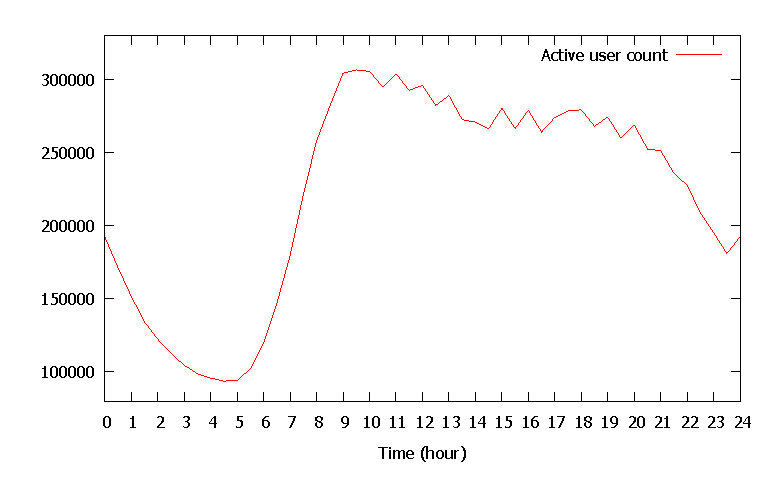
\includegraphics{user_timeslot}
\caption{Active user count over time}
\label{interest:fig:usercount}
\end{figure}

实验中使用不同的抽样方法生成了多个子数据集供训练和测试。除了完整数据集之外,通过随机抽样得到了两个子地理区域,各包含50,000个用户,完整数据集和两个随机抽样数据集分别用$d0$,$d1$及$d2$表示。除了按地理位置随机抽样以外,还将记录按时间来分割,给每个数据集生成了两个子集,分别包含前十天和后十天的记录。每个数据集的两个子集以后缀$-f$和$-l$来分别标识。

\subsection{用户兴趣发现}
实验中使用用户数$U = 469,297$,网站数$W = 924$,以及区域数$R = 265$来进行模型评估。实验中分别在同样的数据集上应用了两种URI模型以及传统LDA模型(使用传统的LDA生成过程)。为了比较,在LDA的抽样过程了,同样记录了每个词所对应的地理区域,而后使用式\ref{interest:equ:phi}来计算一个$K \times R \times W$的$\Phi$的参数矩阵,并使用式\ref{interest:equ:theta2}来计算一个$M \times R \times K$的$\Theta$的参数矩阵,其中$M$为训练集中的用户数。此处,原始的LDA中的$\Phi$和$\Theta$被称为$\Phi0$和$\Theta0$。同时称使用$\Phi0$和$\Theta0$的LDA模型为LDA0,使用$\Phi$和$\Theta0$的模型为LDA1,使用$\Phi0$和$\Theta$的模型为LDA2。
%We also calculated $\Phi0$ for URI model, using the same formula as in LDA:
%\begin{equation}
%	\phi0_{z,w} = \frac{n_{z,*,w} + \beta_w}{\sum_{w'}{(n_{z,*,w'} + \beta_{w'})}}
%\end{equation}
%where $n_{z,\bullet,w}$ means the sum of $n_{z,r,w}$ for each $r \in \mathbf{R}$.

\textbf{评价指标.} 实验中使用``用户兴趣''间的平均Jensen–Shannon差异来评估生成的隐含``兴趣''层的质量。Jensen–Shannon差异(JSD)是评价描述同一随机变量的概率分布间的相似度的常用方法。使用不同的$\Phi$和$\Theta$矩阵作为参数,就能够算出每个模型的JSD。
对于LDA1模型和URI1模型,每个``用户兴趣''内的网站分布于区域有关,JSD的计算方法是:
\begin{equation}
	JSD = \frac{\sum^T_{i=0}\sum^T_{j=i+1}\sum^R_{r=1}{jsd(\mathbf{\phi_{i,r}}, \mathbf{\phi_{j,r}})}}{\frac{T(T+1)}{2} \times R}
\end{equation}
对于其余的模型(LDA0,LDA2以及URI2),JSD的计算方法是:
\begin{equation}
	JSD = \frac{\sum^T_{i=0}\sum^T_{j=i+1}{jsd(\mathbf{\phi0_{i}}, \mathbf{\phi0_{j}})}}{\frac{T(T+1)}{2}}
\end{equation}


为评估模型重现真实的用户行为的能力,实验使用前10天范围内的数据(后缀为\textit{-f}的数据子集)来进行模型训练,而后使用同一数据集的另一数据子集(后缀为\textit{-l})来进行测试(关于数据集的描述参见第\ref{interest:sec:expdata}章)。

所有上述描述的模型均用于估计用户在测试集中的网站访问情况。
使用$d-f$表示训练集,$d-l$来表示测试机,用户$u$在数据集$d-l$中的实际网站分布为:
\begin{equation}
	\widetilde{pl}_{u,w} = \frac{cl_{(u,w,\bullet})}{cl_{(u,\bullet,\bullet)}}
\end{equation}
其中$cl_{u,w,r}$表示数据集$d-l$中,网站$w$在区域$r$内被用户$u$访问的情况($\bullet$表示$所有$)。 

将地理位置信息视为用户的上下文,每个用户的实际地理位置分布为:

\begin{equation}
	\widetilde{ql}_{u,r} = \frac{cl_{u,\bullet,r}}{cl_{u,\bullet,\bullet}}
\end{equation}
 
使用$\Theta$和$\Phi$,能够得到模型输出的估计的分布:
对于LDA1模型和URI1模型:
\[
	p_{u,w} = \sum_i{\left(\theta_{u,i}  \sum_r{(\phi_{i,r,w} \times ql_{u,r})}\right)}
\]
对于LDA2和URI2模型:
\[
	p_{u,w} = \sum_r{\left(\sum_i{\theta_{u,r,i} \times \phi_{i,w}} \times ql_{u,r})\right)}
\]
对于传统LDA模型(不考虑地理位置信息):
\[
	p_{u,w} = \sum_i{(\theta_{u,i} \times \phi_{i,w})}
\]

%For comparison, we also use the distribution of user $u$ on the complete dataset (containing both \textit{-f} and \textit{-l}) to infer $\widetilde{pl}_{u,r}$. In this case, the estimated distributions (with and without considering location) can be calculated as:
%\begin{equation}
%	p_{u,w} = \sum_r{\left(\frac{c_{(u,w,r)}}{c_{(u,\bullet,r)}} \times \widetilde{ql}_{u,r}\right)}
%\end{equation}
%\begin{equation}
%	p0_{u,w} = \frac{c_{(u,w,\bullet)}}{c_{(u,\bullet,\bullet)}}
%\end{equation}
%where $c_{(u,w,r)}$ means the same as $cl_{(u,w,r)}$, except in the complete dataset.

估计得到的用户的网站分布可以看成是他们对于网站的(潜在)偏好,这些信息可被用来理解用户行为模式,也可以用来进行推荐。实验中使用混乱度(perplexity)来评估这些模型生成的概率分布的表现。Perplexity是评估一个估计的概率分布还原真实分布(预测真实分布的样本)能力的常用度量方法。其定义为:
\[
perp(\mathbf{\widetilde{p}},\mathbf{q}) = 2^{H(\mathbf{\widetilde{p}},\mathbf{q})},
\]
其中指数$H(\widetilde{p},q)$为交互熵:
\[
H(\mathbf{\widetilde{p}},\mathbf{q}) = - \sum_x{\widetilde{p}(x)log_2^{q(x)}}
\]
Perplexity的值越小,表明预测的效果越好。所有用户的perplexity的平均值定义为模型输出的概率分布的perplexity值。

%We calculated the self-perplexity of $\widetilde{pl}$, and use it as a (over fitting) standard. The perplexity $perp(\widetilde{pl},\mathbf{pr0})$ of LDA is regarded as baseline. %For clearance, we define a Normalized Reversed Perplexity (NRP) of a proposed distribution $\mathbf{p}$ as:
%\begin{equation}
%	NRP(\mathbf{p}) = \frac{perp(\mathbf{\widetilde{pl}}, \mathbf{pr0_{LDA}}) - perp(\mathbf{\widetilde{pl}}, \mathbf{p})}{perp(\mathbf{\widetilde{pl}}, \mathbf{pr0_{LDA}}) - perp(\mathbf{\widetilde{pl}}, \mathbf{\widetilde{pl}})}
%\end{equation}

\textbf{话题(``用户兴趣'')数.} 实验中尝试了不同的``用户兴趣''(话题)数目$K$。总体来说,还原表现随着$K$的增大的好转(perplexity值下降),而当$K$达到某一值之后趋于稳定;而``用户兴趣''质量则随着$K$的增大的下降($JSD$值随$K$值增大而减小)。实验结果见图\ref{interest:fig:k}。

\begin{figure}
\centering
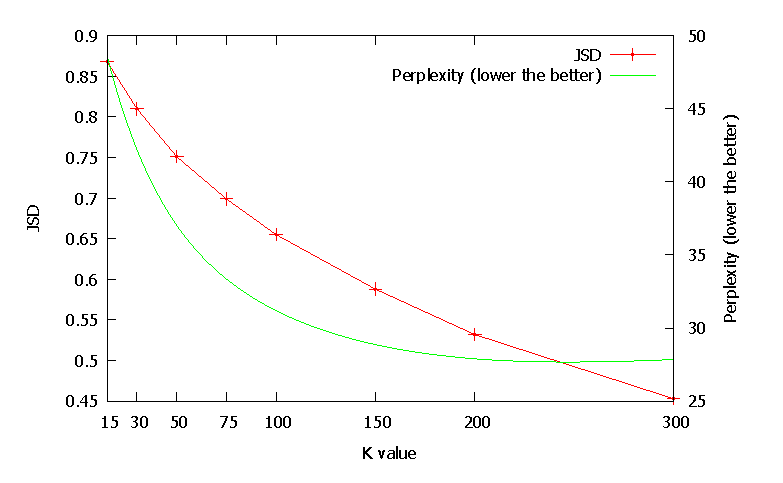
\includegraphics{k}
\caption{不同的\textit{K}值对应的JSD和Perplexity值(URI1模型)}
\label{interest:fig:k}
\end{figure}

同时考虑到模型的泛化能力和重现能力,$JSD$和$Perplexity$是首要关心的指标。在最终实验中选择了$K = 50$作为模型参数。

表\ref{interest:tab:res}展示了所有模型在三个不同数据集上的表现情况。

\begin{table}
\centering
\caption{LDA和URI模型的表现}
\label{interest:tab:res}
\begin{tabular}{|c|c|r|r|} \hline
数据集 & 模型名称 & JSD & Perplexity\\ \hline
\multirow{5}{*}{D0} & LDA0 & 0.040 & 203.805\\ \cline{2-4}
 & LDA1 & 0.211 & 181.824\\ \cline{2-4}
 & LDA2 & 0.211 & 181.824\\ \cline{2-4}
 & URI1 & 0.925 & 98.229\\ \cline{2-4}
 & URI2 & 0.979 & 103.498\\ \cline{2-4}
\hline
\multirow{5}{*}{D1} & LDA0 & 0.079 & 183.021\\ \cline{2-4}
 & LDA1 & 0.307 & 89.910\\ \cline{2-4}
 & LDA2 & 0.990 & 69.853\\ \cline{2-4}
 & URI1 & 0.751 & 34.423\\ \cline{2-4}
 & URI2 & 0.981 & 73.668\\ \cline{2-4}
\hline
\multirow{5}{*}{D2} & LDA0 & 0.064 & 305.282\\ \cline{2-4}
 & LDA1 & 0.247 & 158.881\\ \cline{2-4}
& LDA2 & 0.992 & 64.621\\ \cline{2-4}
 & URI1 & 0.818 & 54.079\\ \cline{2-4}
& URI2 & 0.974 & 121.978\\ \cline{2-4}
\hline\end{tabular}
\end{table}


\section{讨论}
\label{interest:sec:discussion}
本章给出了URI模型及实验结果的讨论,包含实验的结果分析以及给予实验结果的群体行为模式的聚合分析。

\subsection{模型表现分析}
从表\ref{interest:tab:res}中可以看出,总体来说,URI模型的表现显著高于LDA模型。URI2模型发现的隐含``用户兴趣''质量更高,反映出了网站的聚类;而URI1模型能更好的估计每个用户的移动互联网使用行为。这种模型表现可以如下解释:由于URI2中,将地理位置信息作为生成``用户兴趣''时的参数,所以网站在每个``用户兴趣''内的分布与位置无关,而每个``用户兴趣''在每个区域上有一个分布。这就能够更好地将网站聚类,并且将地理位置作为网站类簇的一个特征;另一方面,对于URI1模型,每个网站包含了更多的位置信息,所以其可以更好的估计原始的网站访问分布。由于实验中使用的训练集和测试集时间跨度不大(为连续的时间段),故URI1模型的还原表现更好。

\subsection{群体行为模式聚合分析}
群体行为模式分析,与单个用户的关联较少,与网站的关联较大,如本章中使用URI2模型进行讨论分析。

表\ref{interest:tab:topics}中展示了5个常见的``用户兴趣''及其对应的主题网站。表中还列出了每个用户兴趣的比重,每个用户兴趣中列'出了前5的网站(及其所占比重)作为主题网站。
\begin{table*}
\centering
\caption{URI2模型中的隐含 用户兴趣 层示例}
\label{interest:tab:topics}
\begin{tabular}{|c|r|c|r|c|r|c|r|c|r|} \hline
 \multicolumn{2}{|c|}{兴趣 0} & \multicolumn{2}{|c|}{兴趣 1} & \multicolumn{2}{|c|}{兴趣 2}  \\ \hline
 \multicolumn{2}{|c|}{0.1100} & \multicolumn{2}{|c|}{0.1083} & \multicolumn{2}{|c|}{0.0778}  \\ \hline
weixin.qq.com & 0.8447 & 新浪微博.cn & 0.6761 & z.qq.com & 0.2882\\ \hline
163.com & 0.1424 & sina.cn & 0.3225 & 3g.qq.com & 0.1354 \\ \hline
umeng.com & 0.0059 & 新浪微博.com & 0.0006 & qq.com:8080 & 0.1243\\ \hline
codoon.com & 0.0017 & qik.com & 0.0003 & imtt.qq.com & 0.1115\\ \hline
126.net & 0.0009 & sinaimg.cn & 0.0003 & wap.soso.com & 0.0481\\ \hline

\hline\end{tabular}
\begin{tabular}{|c|r|c|r|} \hline
 \multicolumn{2}{|c|}{兴趣 3} & \multicolumn{2}{|c|}{兴趣 4} \\ \hline
 \multicolumn{2}{|c|}{0.0712} & \multicolumn{2}{|c|}{0.0668} \\ \hline
ucweb.com & 0.3402 & 人人网.com & 0.7282\\ \hline
m.baidu.com & 0.2633 & sina.com.cn & 0.1551\\ \hline
uc.cn & 0.1180 & mafengwo.cn & 0.0599\\ \hline
ucweb.com:80 & 0.0289 & vlingo.com & 0.0212\\ \hline
wap.baidu.com & 0.0253 & emoney.cn & 0.0081\\ \hline

\hline\end{tabular}
\end{table*}

从表中可以看出, 每个``用户兴趣''的主题网站比较集中。兴趣 0 主要是关于\textit{微信},这一当前国内最热门的移动社交应用。这一兴趣同样包含\textit{网易}所提供的门户以及邮箱服务,这说明\textit{微信}用户和\textit{网易}用户的重合度相对更高。兴趣 1 主要包含\textit{微博}这一国内最热门的微博服务。兴趣 2 主要包括\textit{QQ},以及\textit{腾讯}的搜索引擎服务\textit{SOSO}。兴趣 2 的集中性并不十分明显,这是由于\textit{腾讯}提供的服务种类很多,而且他们之间的用户重合度很高。之所以\textit{微信}没有和腾讯其他服务被归到一个兴趣中,是因为\textit{微信}有相对独立的生态系统,与其他腾讯服务的整合度并不太高,而且微信所占的移动互联网使用太高,所以被单独分到一个兴趣之中。兴趣 3 主要包含\textit{百度}以及\textit{UC},这也说明百度的移动客户端并不十分强势,移动流量主要来源于手机浏览器。兴趣 4 主要是关于\textit{人人网},这是一个当前国内(特别是学生中)较为流行的社交网站。

可以看出,``用户兴趣''具有较高的内聚度,能够很好地反映出用户的移动互联网使用行为模式。

经过地理区域发现过程后,数据集中共有265个地理区域。``用户兴趣''在地理区域上的分布$\Psi$计算方式如下:
\[
\psi_{r,z} = \frac{\sum_u{m_{u,r,z}} + \alpha_z}{\sum_{z'}{(\sum_u{m_{u,r,z'}} + \alpha_{z'})}}
\]
其中$m_{u,r,z}$的意义见式\ref{interest:equ:theta2}。

所有区域在数据集上的真实分布记为$\mathbf{ql}$。作为案例研究,表\ref{interest:tab:locs}中展示了两个高热度区域内的主要``用户兴趣''类型。类似表\ref{interest:tab:topics},展示了区域及其频度,以及其排名前五的``用户兴趣''的ID、内容(总结自其主题网站)和在此区域内的频度。

\begin{table}
\centering
\caption{两个示例区域内的 用户兴趣 分布}
\label{interest:tab:locs}
\begin{tabular}{|c|c|c|r|c|c|r|} \hline
 \multicolumn{3}{|c|}{区域 58} & \multicolumn{3}{|c|}{ 区域 0} \\ \hline
 \multicolumn{3}{|c|}{0.0210} & \multicolumn{3}{|c|}{  0.0178} \\ \hline
1 & 新浪微博 & 0.1542 & 0 & 微信 & 0.0971\\ \hline
 0 & 微信 & 0.1120 & 5 & 人人网 & 0.0957\\ \hline
 8 & Apple & 0.0863 & 1 & 新浪微博 & 0.0908\\ \hline
 3 & QQ门户 & 0.0727 & 4 & UC \& Baidu & 0.0844\\ \hline
 5 & 人人网 & 0.0619 & 2 & QQ(腾讯) & 0.0837\\ 
\hline\end{tabular}
\end{table}

区域 58 是一个商业区,该区域内的活跃用户为白领上班族;区域 0 是一个学校区域,该区域内有若干高校,活跃用户主要是高校学生。从表\ref{interest:tab:locs}可以清楚地看到这两个区域在兴趣分布上的区别:在区域 58 中,新浪微博的比重显著高于区域 0,这表明新浪微博在白领中的流行度更高;相反,\textit{人人网}在区域 0 中的比重更高,这说明该服务在高校学生中更为流行。这些发现与根据实际情况的猜想是一致的。

这两个区域的另一个区别在于\textit{苹果公司}网站的比重。这些网站在区域 58 内排名第3,而在区域 0 内却没有排进前5。这说明苹果设备在中国的白领之中市场占有率要普遍高于学生。由于iPhone等苹果设备在中国属于近似奢侈品,价格昂贵,所以其在白领中的受欢迎度更高,白领的购买能力也更强,这一结论也和实际情况比较一致。

\section{本章小结}
\label{interest:sec:conclusion}
本章提出了基于运营商数据进行用户移动互联网上网行为分析的方法。提出了一个根据地点的移动互联网流量来将其划分为地理功能区域的聚类方法;提出了基于概率话题模型的方法,来从移动互联网使用记录中,联系地理区域信息,解析出隐含的``用户兴趣''层。共提出了两个话题模型,并分别将其应用于北京地区的真实运营商数据集,其中覆盖了超过三百万的用户。实验结果表明,模型具有较好的有效性和还原(预测)能力。模型输出了有意义的和用户行为模式。根据模型输出进行了城市级别的聚合用户行为模式的分析,并讨论了不同地理功能区域之间的对比差异。

